\documentclass[14pt,fleqn]{extarticle}
\RequirePackage{prepwell}
\previewoff


\newcommand\ysq{\left(\frac{9}{4}-x^2 \right)}
\newcommand\xsq{\left(\frac{3}{2} \right)^2 - y^2}
\newcommand\intg{2\int_{0}^{\sqrt{2}}}

\begin{document}

%text
Find the area of the circle $4x^2+4y^2=9$ 
which is interior to the parabola $x^2=4y$.
%

\newcard

\begin{center}
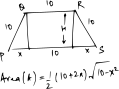
\includegraphics[scale=1.3]{img_prefab-1.svg} 
\end{center} 

\newcard

\begin{center}
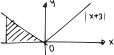
\includegraphics[scale=1.3]{img_prefab-2.svg} 
\end{center} 

\newcard

\[ 4x^2 + 4y^2 = 9 \implies \underbrace{x^2 + y^2 = \left(\frac{3}{2} \right)^2}_{\text{Standard form}} \]

Only from the standard form can one infer the center and radius of the circle. And we can see that the circle is centered at $(0,0)$ and has $R = \frac{3}{2}$ \newline 

The parabola $y = \frac{x^2}{4}$ opens upwards. Note that $ y\geq 0$ for all $x$ \newline 

The required area has to be \underline{inside both}  the circle \& the parabola\newline 

Hence, it must be as shown in the figure below 

\begin{center}
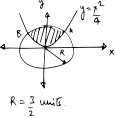
\includegraphics[scale=1.3]{circ.svg} 
\end{center} 

\newcard 

The parabola and the circle intersect at 
\[ \quad  A =\left(\sqrt{2},\frac{1}{2} \right) \text{ and }B = \left( -\sqrt{2},\frac{1}{2}\right) \]

\newcard 

The parabola and the circle intersect at 
\[ A = \left( 1,\frac{\sqrt{5}}{2} \right) \text{ and } B = \left(-1,\frac{\sqrt{5}}{2} \right)  \]

\newcard 

The parabola and the circle will intersect when 

\begin{align}
x^2 = \underbrace{\xsq}_{\text{Circle}} &= \underbrace{4y}_{\text{Parabola}} \\
\implies 4y^2 + 16y - 9 &= 0 \\
\text{or }(2y+9)\cdot (2y-1) &= 0\implies y=-\frac{9}{2},\frac{1}{2}
\end{align}

But \underline{$y > 0$} for both $A$ and $B$ -- as can be seen from the figure 
%
\begin{align}
\text{Hence, }x^2 &= 4y = 4\cdot\frac{1}{2} = 2 \\
\implies x &= \pm\sqrt{2} \\
\implies A &=\left(\sqrt{2},\frac{1}{2} \right) \text{ and }B = \left( -\sqrt{2},\frac{1}{2}\right)
\end{align}


\newcard 

The required area $R$ will be 
\[ \quad R = \intg \left[\sqrt{\ysq} - \frac{x^2}{4} \right]\cdot dx \]

\newcard 
The required area $R$ will be 
\[ \quad R = \intg \left[\frac{x^2}{4} - \sqrt{\ysq}\right]\cdot dx \]

\newcard 

In the range $x=-\sqrt{2}\rightarrow x=\sqrt{2}$, the 
\underline{circle lies above the parabola}. Hence, the
required area $R$ will be given by 

\begin{align}
R &= \int_{-\sqrt{2}}^{\sqrt{2}}\left( \sqrt{\frac{9}{4}-x^2} - \frac{x^2}{4}\right)\cdot dx
\end{align} 

But notice that the circle, the parabola and the required area $R$ are all \underline{symmetrical} about the $y-$axis\newline 

Hence, we can also say that 
\[ \quad R = \intg \left( \sqrt{\frac{9}{4}-x^2} - \frac{x^2}{4}\right)\cdot dx \]

\newcard 
\[ \qquad R = \frac{9}{4}\sin^{-1}\frac{2\sqrt{2}}{3} + \frac{1}{3\sqrt{2}} \]

\newcard 

\begin{align}
	R &= \underbrace{\intg \sqrt{\ysq}\cdot dx}_P - \underbrace{\intg \frac{x^2}{4}\cdot dx}_Q \\ 
	P &= \underbrace{\intg \sqrt{\left(\frac{3}{2} \right)^2 - x^2}\cdot dx }_{a = \frac{3}{2}} \\
	&= 2\cdot\left[ \frac{a^2}{2}\sin^{-1}\frac{x}{a}+ \frac{x}{2}\sqrt{a^2-x^2}\right]_0^{\sqrt{2}} \\
	&= 2\cdot\left[ \left(\frac{\frac{9}{4}}{2}\sin^{-1}\frac{\sqrt{2}}{\frac{3}{2}}+
\frac{\sqrt{2}}{2}\sqrt{\frac{9}{4}-2}\right)- 0\right] \\
&= \frac{9}{4}\sin^{-1}\frac{2\sqrt{2}}{3} + \sqrt{2}\frac{1}{2} \\
&=  \frac{9}{4}\sin^{-1}\frac{2\sqrt{2}}{3} + \frac{1}{\sqrt{2}} \\
Q &= 2\int_0^{\sqrt{2}}\frac{x^2}{4}\cdot dx = \left[ \frac{x^3}{6}\right]_0^{\sqrt{2}} = \frac{\sqrt{2}}{3} \\
\therefore R &= \frac{9}{4}\sin^{-1}\frac{2\sqrt{2}}{3} + 
\underbrace{\frac{1}{\sqrt{2}}- \frac{\sqrt{2}}{3}}_{\text{Simplify}} \\
&= \frac{9}{4}\sin^{-1}\frac{2\sqrt{2}}{3} + \frac{1}{3\sqrt{2}}
\end{align}


\end{document}
